\documentclass[a4paper,12pt]{article}
\usepackage[left=2.5cm,right=2.5cm,top=2.5cm,bottom=2.5cm]{geometry} % Adjust page margins
\usepackage{xcolor,graphicx,framed}
\usepackage[normalem]{ulem}
\usepackage{amsmath}
\usepackage{gensymb}
%\usepackage{lastpage} % Required to print the total number of pages

\begin{document}

\newcommand{\HRule}{\rule{\linewidth}{0.4mm}} % Defines a new command for the horizontal lines, change thickness here

%----------------------------------------------------------------------------------------
%	HEADING SECTIONS
%----------------------------------------------------------------------------------------

\begin{minipage}{0.7\textwidth}
\begin{flushleft} 
\textsc{Universidad del Valle de Guatemala \\
Campus Central \\
Facultad de Ciencias y Humanidades \\
Departamento de Qu\'imica \\
Segundo ciclo, 2014 \\
Fisicoqu\'imica 1 \\
}
\end{flushleft}
\end{minipage}
~
\begin{minipage}{0.2\textwidth}
\begin{flushright}

\includegraphics[scale=0.3]{Logo_UVG} % Include a department/university logo
\end{flushright}
\end{minipage}\\

%----------------------------------------------------------------------------------------
%	TITLE SECTION
%----------------------------------------------------------------------------------------

\begin{center}
\HRule \\[0.4cm]
{ \bfseries Soluciones propuestas a los ejercicios en clase, 2}\\ % Title of your document
\HRule \\[0.4cm]
\end{center}

%----------------------------------------------------------------------------------------

\begin{enumerate}

 \item \textbf{\textit{(McQuarrie 16-58)} El coeficiente de dilataci\'on t\'ermica (coefficient of thermal expansion), $\alpha$, est\'a definido como:
$$\alpha=\frac{1}{\bar{V}}\left(\frac{\partial \bar{V}}{\partial T}\right)_P$$
Mostrar que para un gas ideal $\alpha=\frac{1}{T}$.} % Problema 2-58

Como se tiene que calcular la derivada parcial de $\bar{V}$ con respecto a $T$, expresamos una en t\'erminos de la otra:
$$PV=nRT\rightarrow \bar{V}=\frac{RT}{P}$$
Calculando la derivada parcial:
$$\frac{\partial \bar{V}}{\partial T}=\frac{\partial }{\partial T}\left(\frac{RT}{P}\right)=\frac{R}{P}$$
Entonces:
$$\alpha=\frac{1}{\bar{V}}\left(\frac{\partial \bar{V}}{\partial T}\right)_P=\frac{1}{\bar{V}}\frac{R}{P}=\frac{P}{RT}\frac{R}{P}=\frac{1}{T}$$

 \item \textbf{\textit{(McQuarrie 16-59)} La compresibilidad isoterma (isothermal compressibility), $\kappa$, est\'a definida como:
$$\kappa=-\frac{1}{\bar{V}}\left(\frac{\partial \bar{V}}{\partial P}\right)_T$$
Mostrar que para un gas ideal $\kappa=\frac{1}{P}$.} % Problema 2-59

Usando la expresi\'on anterior de $\bar{V}$, podemos calcular la derivada parcial:
$$\frac{\partial \bar{V}}{\partial P}=\frac{\partial }{\partial T}\left(\frac{RT}{P}\right)=-\frac{RT}{P^2}$$
Entonces:
$$\kappa=-\frac{1}{\bar{V}}\left(\frac{\partial \bar{V}}{\partial P}\right)_T=-\left(\frac{1}{\bar{V}}\right)\left(-\frac{RT}{P^2}\right)=\frac{P}{RT}\frac{RT}{P^2}=\frac{1}{P}$$

\newpage

 \item \textbf{\textit{(McQuarrie 16-17)} Usar la ecuaci\'on de van der Waals para calcular la presi\'on de un mol de etano a $400.0\;\mbox{K}$ confinado a un volumen de $83.26\;\mbox{cm}^3$. El valor experimental es $400\;\mbox{bar}$.} % Problema 2-17

La ecuaci\'on de van der Waals es:
$$\left(P+\frac{a}{\bar{V}^2}\right)\left(\bar{V}-b\right)=RT\rightarrow P=\frac{RT}{\bar{V}-b}-\frac{a}{\bar{V}^2}$$
Como es un mol de etano, el volumen molar es: 
$$\bar{V}=V/n=83.26\;\mbox{cm}^3\left(\frac{1.00\;\mbox{dm}^{3}}{1000\;\mbox{cm}^{3}}\right)/(1\;\mbox{mol})=8.326\times 10^{-2}\;\mbox{dm}^3\cdot\mbox{mol}^{-1}$$
Para etano tenemos $a=5.5818\;\mbox{dm}^6\cdot\mbox{bar}\cdot\mbox{mol}^{-2}$ y $b=0.065144\;\mbox{dm}^3\cdot\mbox{mol}^{-1}$, entonces:
$$P=\frac{(8.314\times 10^{-2}\;\mbox{dm}^3\cdot\mbox{bar}\cdot\mbox{K}^{-1})(400.0\;\mbox{K})}{8.326\times 10^{-2}\;\mbox{dm}^3\cdot\mbox{mol}^{-1}-0.065144\;\mbox{dm}^3\cdot\mbox{mol}^{-1}}-\frac{5.5818\;\mbox{dm}^6\cdot\mbox{bar}\cdot\mbox{mol}^{-2}}{\left(8.326\times 10^{-2}\;\mbox{dm}^3\cdot\mbox{mol}^{-1}\right)^2}$$
Lo que da un valor de $P=1030\;\mbox{bar}$, que, comparado con el valor experimental, no es un buen resultado.

 \item \textbf{\textit{(McQuarrie 16-22)} Mostrar que la ecuaci\'on de van der Waals para el Arg\'on a $T=142.69\;\mbox{K}$ y $P=35.00\;\mbox{atm}$ puede ser escrita como:
$$\bar{V}^3-0.3664\bar{V}^2+0.03802\bar{V}-0.001210=0$$} % Problema 2-22

De primero, tratemos de despejar $\bar{V}$ en la ecuaci\'on de van der Waals:
$$\left(P+\frac{a}{\bar{V}^2}\right)\left(\bar{V}-b\right)=RT\rightarrow P\bar{V}-Pb+\frac{a}{\bar{V}}-\frac{ab}{\bar{V}^2}=RT$$
$$\rightarrow \bar{V}-b+\frac{a}{P\bar{V}}-\frac{ab}{P\bar{V}^2}-\frac{RT}{P}=0$$
$$\rightarrow \bar{V}^3-b\bar{V}^2+\frac{a}{P}\bar{V}-\frac{ab}{P}-\frac{RT}{P}\bar{V}^2=0$$
$$\rightarrow \bar{V}^3-\left(b+\frac{RT}{P}\right)\bar{V}^2+\frac{a}{P}\bar{V}-\frac{ab}{P}=0$$
Convirtiendo la presi\'on a $\mbox{bar}$, tenemos:
$$P=35.00\;\mbox{atm}\left(\frac{1.01325\;\mbox{bar}}{1\;\mbox{atm}}\right)=35.46\;\mbox{bar}$$
Para Arg\'on tenemos $a=1.3483\;\mbox{dm}^6\cdot\mbox{bar}\cdot\mbox{mol}^{-2}$ y $b=0.031830\;\mbox{dm}^3\cdot\mbox{mol}^{-1}$, entonces:
\begin{align*}
\bar{V}^3& -\left(0.031830\;\mbox{dm}^3\cdot\mbox{mol}^{-1}+\frac{(8.314\times 10^{-2}\;\mbox{dm}^3\cdot\mbox{bar}\cdot\mbox{K}^{-1})(142.69\;\mbox{K})}{35.46\;\mbox{bar}}\right)\bar{V}^2+ \\
& \left(\frac{1.3483\;\mbox{dm}^6\cdot\mbox{bar}\cdot\mbox{mol}^{-2}}{35.46\;\mbox{bar}}\right)\bar{V}-\frac{(1.3483\;\mbox{dm}^6\cdot\mbox{bar}\cdot\mbox{mol}^{-2})(0.031830\;\mbox{dm}^3\cdot\mbox{mol}^{-1})}{35.46\;\mbox{bar}}=0
\end{align*}
Lo que da, luego de hacer las operaciones para obtener los coeficientes:
$$\bar{V}^3-(0.3664\;\mbox{dm}^3\cdot\mbox{mol}^{-1})\bar{V}^2+(0.03802\;\mbox{dm}^6\cdot\mbox{mol}^{-2})\bar{V}-0.001210\;\mbox{dm}^9\cdot\mbox{mol}^{-3}=0$$

 \item \textbf{\textit{(McQuarrie 16-15)} Usar la ecuaci\'on de van der Waals para calcular el volumen molar de $CO$ a $200\;\mbox{K}$ y $1000\;\mbox{bar}$. Comparar el resultado con lo que obtendr\'ian usando la ecuaci\'on del gas ideal. El valor experimental es $0.04009\;\mbox{L}\cdot\mbox{mol}^{-1}$.} % Problema 2-15

Para $CO$ tenemos $a=1.4734\;\mbox{dm}^6\cdot\mbox{bar}\cdot\mbox{mol}^{-2}$ y $b=0.039523\;\mbox{dm}^3\cdot\mbox{mol}^{-1}$. Usando la ecuaci\'on del ejercicio anterior:
\begin{align*}
\bar{V}^3 &-\left(0.039523\;\mbox{dm}^3\cdot\mbox{mol}^{-1}+\frac{(8.314\times 10^{-2}\;\mbox{dm}^3\cdot\mbox{bar}\cdot\mbox{K}^{-1})(200\;\mbox{K})}{1000\;\mbox{bar}}\right)\bar{V}^2+ \\
& \left(\frac{1.4734\;\mbox{dm}^6\cdot\mbox{bar}\cdot\mbox{mol}^{-2}}{1000\;\mbox{bar}}\right)\bar{V}-\frac{(1.4734\;\mbox{dm}^6\cdot\mbox{bar}\cdot\mbox{mol}^{-2})(0.039523\;\mbox{dm}^3\cdot\mbox{mol}^{-1})}{1000\;\mbox{bar}}=0
\end{align*}
Lo que da:
$$\bar{V}^3-(0.056151\;\mbox{dm}^3\cdot\mbox{mol}^{-1})\bar{V}^2+(0.0014734\;\mbox{dm}^6\cdot\mbox{mol}^{-2})\bar{V}-5.82332\times10^{-5}\;\mbox{dm}^9\cdot\mbox{mol}^{-3}=0$$
Cuya gr\'afica es:
\begin{center}
 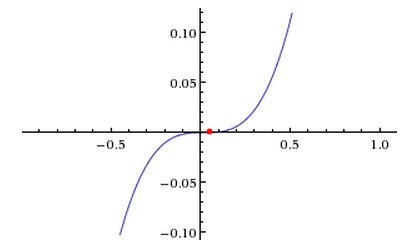
\includegraphics[scale=0.7]{figure2}
\end{center}
Para determinar el volumen molar, necesitamos determinar los ceros de la ecuaci\'on. Usando alguna herramienta matem\'atica, se determina que el \'unico cero real de esa ecuaci\'on es $\bar{V}=0.04998\;\mbox{dm}^3\cdot\mbox{mol}^{-1}$, cercano al valor experimental.

\end{enumerate}
 
\end{document}
